\documentclass[11pt]{article}

\usepackage{graphicx}
\usepackage{tikz}
\usetikzlibrary{shapes.geometric, arrows}
\tikzstyle{recNode} = [rectangle, minimum width=3cm, minimum height=1cm, text centered, draw=black]
\tikzstyle{eNode} = [minimum height=1cm, text centered]
\tikzstyle{arrow} = [thick,->,>=stealth]

\usepackage{etoolbox}
\patchcmd{\thebibliography}{\section*}{\section}{}{}

\author{Hodai Goldman (Hodaig@cs.bgu.ac.il) \\
Department of Computer Science, \\
Ben-Gurion University of the Negev, Beer Sheva, Israel \\
Supervisor: Dr. Gera Weiss}
\date{\today}
\title{Research Proposal: Computational resource management of multi channel controller}

\begin{document}
\begin{titlepage}
\maketitle
\end{titlepage}




\section{Background and Problem Formulation}
\label{sec:Background}
Today's computer power allows for consolidation of controllers where a single computer can regulate many control loops, each with its varying needs of computation resources.
This brings two research challenges that we intend to attack in the proposed thesis:
\begin{itemize}
	\item How to schedule control tasks in order to achieve good performance in terms of control measures (overshoot, convergence speed, etc.)?
	\item What is a good interface for co-design of scheduling and control?
\end{itemize}

While it is possible to build control systems using standard operating systems, either real-time or desktop with static or with dynamic scheduling schemes, there is an agreed opinion in the control community that these do not serve well for the purpose outlined above~\cite{??}. Specifically, desktop type operating systems (Windows, Linux, etc.) schedule for computational efficiency, but do not allow for control performance guarantees of the individual loops. On the other hand, real-time operating systems sacrifice some efficiency for timing predictability, but they do relate timing information with control performance. When using such operating systems for control engineers usually apply controllers that work in a fixed periodic manner so that control behavior becomes deterministic and control performance can be guaranteed. This is not efficient because resources can be better utilized if controllers act at higher frequencies when only when needed. 
In this work we will develop methods to combine the efficiency of desktop operating systems with the predictability of real-time operating systems in a way that is more suitable for control systems then periods and deadlines

%Although scheduling is a well researched area, covered in many research papers and books, existing scheduling theory is not yet fully adopted to work in the context of control systems~\cite{?}.
%In the engineering practice, typically, scheduling mechanisms can be characterized as one of two types:
%\begin{description}
%	\item[Dynamic Schedule:]{
%		a commonly uses scheduling method in desktop operation systems (eg. Windows, Linux) that aims at efficiency of CPU usage.
%	}
%	
%	\item[Real-Time schedule:]{
%		such as embedded systems for automatic control (for example robotics), 
%		scheduling is guided by specifications of \textbf{periods} and \textbf{deadlines}, the scheduler must ensure that processes can meet deadlines. this limitations are for keeping the system stable but usually not efficient.
%	}
%\end{description}
%in this thesis we will suggest a technique to combine the efficiency of desktop operating systems with the predictability of real-time operating systems,
%in a way that is more suitable for control systems then periods and deadlines (see section TODO ).

The control loops that we are analyzing are here of the form shown in Figure~\ref{fig:control loop}. A physical plant (controlled system) is connected via sensors and actuators... % TODO - Gera: explain the figure

The current state of the art is that control engineers design control tasks as periodic computations then they specify the required periodic frequency for the task and software engineers design a scheduler that ensures that the periodic frequency requirements are met usually using pre-computed knowledge of the expected (maximum) duration of the tasks.
We claim that for control systems we can achieve better performance by using richer and more flexible set of requirements for the tasks. Specifically, we will develop tools with which the control engineers can specify in a natural way features of their control loop that the scheduler will use to allow for dynamic schedules that guarantee required control performance. 

\begin{figure}[]
    \centering
    
    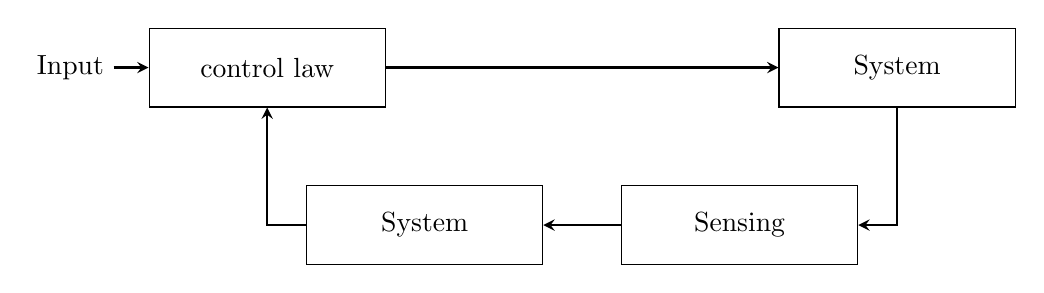
\begin{tikzpicture}[node distance=2cm]
        \node (in) [eNode] {Input};
        \node (control) [recNode, right of=in, xshift=0.5cm] {control law};
        \node (sys) [recNode, right of=control, xshift=6cm] {System};
        \node (sensor) [recNode, below of=sys, xshift=-2cm] {Sensing};
        \node (estimator) [recNode, below of=control, xshift=2cm] {System};
        
        \draw [arrow] (in) -- (control);
        \draw [arrow] (control) -- (sys);
        \draw [arrow] (sys) |- (sensor);
        \draw [arrow] (sensor) -- (estimator);
        \draw [arrow] (estimator) -| (control);
    \end{tikzpicture}
    
    \caption{Typical control loop system.
    \label{fig:control loop}}
\end{figure}

\section{Case study: Vision based controllers for drones}
\label{sec:Case study}
%TODO - hodai: what exactly should i write here?

Tomatoes in green houses require much manual labor such as pollination.
In fields Pollination is done by wind and by wild insects, In green houses by bumble bees or humans. 
Bumbles bees are the most popular In green houses but they are Sensitive to weather (heat) and Sensitive to pesticides.

The leading Case study scenario that we will be examine is a flying drones that will replace the bumbles. 
They goal is top identify the tomatoes flowers in a tomatoes row and then fly near the flowers in order to pollinate them using their natural rotors wind.

This task is very challenging for an autonomous drone, the hall between rows is very tight so the drone must be very stable and mast have accurate knowledge of his own state and location, therefore the drone use vision (cameras) to understand ware he is (state estimation) and to identify the flowers.
This is lead to another challenging task, how can we construct real-time controller with such computational expensive $Computer~Vision$ tasks, without loose the stabilization (predictability) of the system.
Tis is the main issue of this thesis, as show in section \ref{sec:Research Plan}, we suggest a novel framework model for such systems.




\section{Research Plan}
\label{sec:Research Plan}
%In this thesis we suggest a novel technique where the control loop is composed (as usual) from control tasks and state estimation tasks. 
%And the requirement of the periodical requirements of the control tasks dynamically change and depend on the level of the environmental noise that is expressed by the accuracy of the state estimation (retrieve from estimation loops) and the stability of the system (retrieve from the control loop).

\begin{figure}[ht]
%TODO - maybe add \%CPU arrow from scheduler to control law 
%TODO - replace with tikzpicture
  \centering
  \includegraphics[width=0.7\textwidth]{hybrid-loop.png}
  \caption{Our proposal of the controller control system framework
  \label{fig:hybrid loop}}
\end{figure}

\subsection{the controller control system framework}
\label{sec:our proposal}

As show in Figure \ref{fig:hybrid loop} the suggested control system framework have strong relation between the tasks scheduler to the control loops, in this case to the estimation task ($State~Estimation$) and the sensing task ($Computer~Vision$), 
in this framework the scheduler is part of the control logic and therefore it can make scheduling decisions based on the current control state, in the above example (Figure \ref{fig:hybrid loop}) the scheduling of $Computer~Vision$ task is depended on the accuracy of the state estimation.
For example if the vision is clear the $Computer~Vision$ will produce good measurement of the System and therefore good accuracy will be achieved so the $Scheduler$ can allocate less computation time to the heavy $Computer~Vision$ task and still remain stable and allocate more CPU to others control loops or some background tasks (like navigation).

The above collaboration require to re-adjust some parts of the controlling system, e.g. the $State~Estimator$ need to work with variable error of $Computer~Vision$ measurement and the $Computer~Vision$ need to be able to run within variable time limits, and also the tasks pre-defined requirements need to be re-adjust in order to define the relation between the tasks like $Computer~Vision$ and $State~Estimator$.
now we will dive in each part of the above system (Figure \ref{fig:hybrid loop}) and explain how it should be adjusted (changed) and how we will achieve that adjustment in our demonstration (see \ref{sec:Case study}).

Finally, we need to re-consider the system Analyzing technique because variable sensing characteristics ($Computer~Vision$ time limits) will lead to variable estimation characteristics... %TODO - complete and fix this paragraph or remove it

\subsubsection{Sensors ($Computer~Vision~Based~Sensor$)}
\label{sec:sensors}
%Anitime reserch

$Computer~Vision~Based~Sensor$ is the module that responsible to take picture or series of pictures and produce the goal measurement.
For that example we will use the $Computer~Vision$ in order to detect 2 dimensional movement in the camera surface (i.e. the drone speed).
There are lots of such algorithms (optical flow), they differ by their running time and by the accuracy of the solution, mostly more time lead to more accuracy.

In our case we need to be able to control the $Computer~Vision$ running time and to have some god knowledge of the solution accuracy in order to match the correspond state estimation (see \ref{sec:estimator}) logic.
We assume that the $Computer~Vision$ error is spread Normally, this is acceptable assumption because ??? \cite{???}, so we will use the error Covariance as the solution accuracy.

%TODO
In order to control the running time, we will use an Anytime vision algorithms show by ??? \cite{???}.
This type of algorithms will run till we stop them, and wen we stop them they will provide a solution with accuracy that is proportional to the amount of time he was running, that way we can control the solution accuracy by controlling the running time.
In our implementation, in order to lower the complexity, we will pre-define few different operation modes" of the $Computer~Vision$ task, that differ by their running time and they identified by a pair $(RunTime, Covariance)$ where $Covariance$ is the error covariance of running time $RunTime$.

\subsubsection{State Estimator}
\label{sec:estimator}
% kalman filter & ...

\subsubsection{Control Tasks}
%TODO - ???

\subsubsection{Automata Based Scheduler}
%This research continues/completes the work of Merav Bukra ~\cite{Merav} on scheduling computations in embedded control systems.
%In her thesis Merav presented an approach and a proof-of-concept tool for scheduling computation resources in control software. The tool was good enough for demonstrating the concept with simulations, but it did not integrate with any real-life system. In this research we will develop a resource scheduler for real-life control model (see~\ref{sec:contmode}),and upgrade the control software (APM) of a well-known quad-copter by replacing it's RT-scheduler with our new scheduler.
%We expect an improvement in CPU utilization that will allow improvements of stability of the drone.

\subsection{experimental environment}
\subsubsection{drones}
\subsubsection{Ardu-Pilot-Mega as base controller software}

\section{Preliminary Results}
Blablabla said Nobody ~\cite{Merav}.
Blablabla said Nobody ~\cite{APM}.
Blablabla said Nobody ~\cite{RTComposer}.


\begin{samepage}
    \bibliography{proposal}{}
    \bibliographystyle{plain}
\end{samepage}

\end{document}}